\documentclass[12pt, aspectratio=169, abstract=off, oneside]{beamer}
\usepackage{graphicx} % includegraphics
\usepackage{epstopdf} % include *.eps figures in document
\usepackage{textcomp} % text macros (textcelsius, etc.)
%\usepackage{placeins} % forced display for floating objects
\usepackage{indentfirst} % indent first line
\usepackage{hyperref} % links for the table of content
\usepackage{amsmath} % math package
%\usepackage{subfigure} % subfigure package

\usepackage[font=small,labelfont=bf, format=plain]{caption} % caption
\usepackage[utf8]{inputenc} % encodierung
\usepackage[english]{babel} % language
%\usepackage[version=3,arrows=pgf-filled]{mhchem} % chemistry package
%\usepackage{multirow} % multirow in tables
%\usepackage{wrapfig} % enable text wrapping around figures

\usepackage{natbib} % citation
\bibpunct{(}{)}{;}{a}{}{,}  % adjust author-year citation format  


% header and footers
\usepackage{scrpage2} % header and footer 
% \pagestyle{scrheadings}
% \ihead{Left Header} % left header text
% \ohead{Right Header} % right header text

% underscripted equal sign
\newcommand{\underrel}[2]{\mathrel{\mathop{#2}\limits_{#1}}}

% define commands to display derivatives in math mode
\renewcommand{\d}{\mathrm{d}}
\newcommand{\D}{\mathrm{D}}
\newcommand{\dd}[2]{\frac{\mathrm{d} #1}{\mathrm{d} #2}}
\newcommand{\dD}[2]{\frac{\mathrm{D} #1}{\mathrm{D} #2}}
\newcommand{\dpar}[2]{\frac{\partial #1}{\partial #2}}
\newcommand{\dDelta}[2]{\frac{\Delta #1}{\Delta #2}}

% define commands to display units in math mode
\newcommand{\unit}[1]{\mathrm{#1}}
\newcommand{\unitb}[1]{\left[\mathrm{#1}\right]}
\newcommand{\unitf}[2]{\mathrm{\frac{#1}{#2}}}
\newcommand{\unitfb}[2]{\mathrm{\left[ \frac{#1}{#2} \right]}}
\newcommand{\e}[1]{\cdot 10^{#1}}

% commands for reference to floating objects
\newcommand{\tab}[1]{Table \ref{#1}}
\newcommand{\eqn}[1]{Equation (\ref{#1})}
\newcommand{\fig}[1]{Figure \ref{#1}}
\newcommand{\celsius}{\textdegree{}C}
\newcommand{\cms}{$\unit{cms^{-1}}$}

% -------------------------
% start of the document
% -------------------------

\begin{document}

	% title + intro: 
	\title{Volume/area scaling model vs.\\OGGM flowline model}
    \subtitle{A Master's Thesis SITREP}
    \author{Moritz Oberrauch}
    \titlegraphic{\includegraphics[width=0.75\textwidth]{/Users/oberrauch/Desktop/slides/title.jpg}}

    \frame{\titlepage}

    \begin{frame}[t]\frametitle{Introduction}
        \centering
        \includegraphics[width=0.52\textwidth]{/Users/oberrauch/Desktop/slides/watze.jpg}<1>
        \includegraphics[width=0.4\textwidth]{/Users/oberrauch/Desktop/slides/bumiller.jpg}<2>
        \includegraphics[width=0.4\textwidth]{/Users/oberrauch/Desktop/slides/freiger.jpg}<3>
        \includegraphics[width=0.8\textwidth]{/Users/oberrauch/Desktop/slides/fieldwork.jpg}<4>

        \begin{block}{Testing the importance of explicit glacier dynamics for future glacier evolution in the Alps}<5->
        \end{block}
        \begin{block}{\color[HTML]{f69d0e}{How much better is the OGGM really?!}}<6->
            
        \end{block}

        \begin{itemize}
            \item<7-> Ben's original model \citep{Marzeion2012b}
            \item<8-> Implementation
            \item<9-> Comparing/testing against the OGGM flowline model
            \item<10-> Sensitivity analysis
            \item<11-> Future ice volume projection
        \end{itemize}
        
    
    \end{frame}

    \begin{frame}[t]\frametitle{Volume/area scaling model}

        \centering
        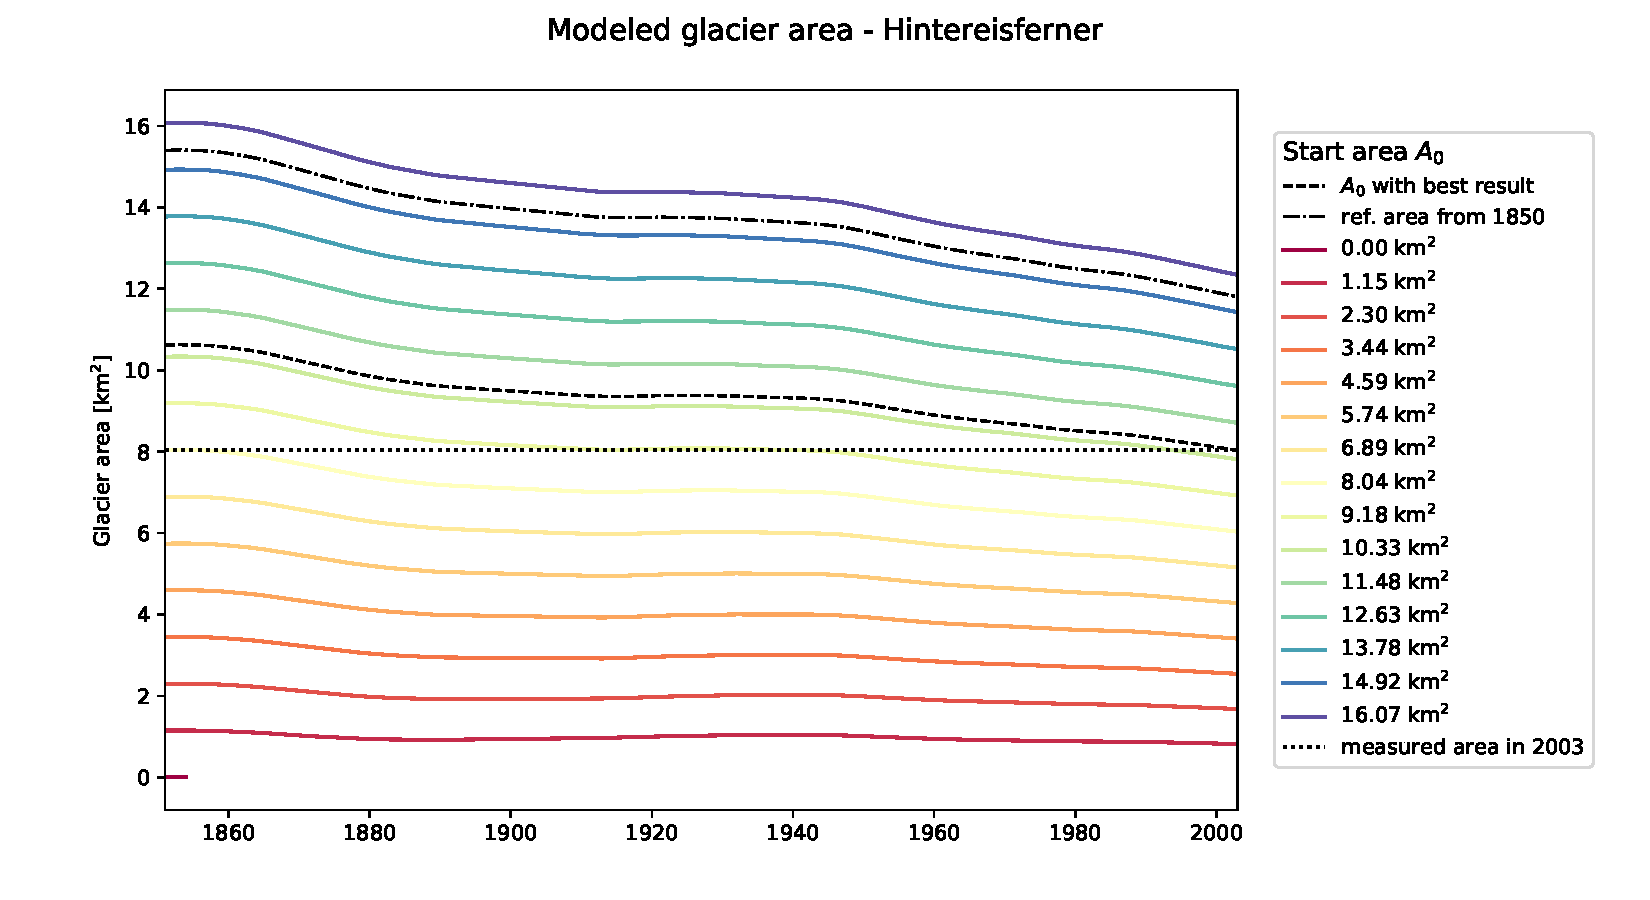
\includegraphics[width=0.9\textwidth]{/Users/oberrauch/Desktop/slides/hintereisferner.jpg}<1>
        \includegraphics[width=0.9\textwidth]{/Users/oberrauch/Desktop/slides/hintereisferner_outline.pdf}<2>
        \includegraphics[width=0.9\textwidth]{/Users/oberrauch/Desktop/slides/hintereisferner_area.pdf}<3>
    
    \end{frame}

    \begin{frame}[t]\frametitle{Volume/area scaling model}
        \centering
        \only<1,3>{Volume/area scaling relation:
        \begin{equation*}
            V_0 = c_A \cdot A_0^\gamma
        \end{equation*}\\}
        \only<2>{
        \vfill
        \includegraphics[width=0.5\textwidth]{/Users/oberrauch/Desktop/slides/cube.pdf}}
        
        \only<3>{
        \vfill
        Inverted volume/length scaling relation:
        \begin{equation*}
            L_0 = \frac{V_0}{c_L}^{1/q}
        \end{equation*}}
        \only<4>{
        \vfill
        \includegraphics[width=0.5\textwidth]{/Users/oberrauch/Desktop/slides/cuboid.pdf}}
    
    \end{frame}

    \begin{frame}[t]\frametitle{Volume/area scaling model}
        
        \centering
        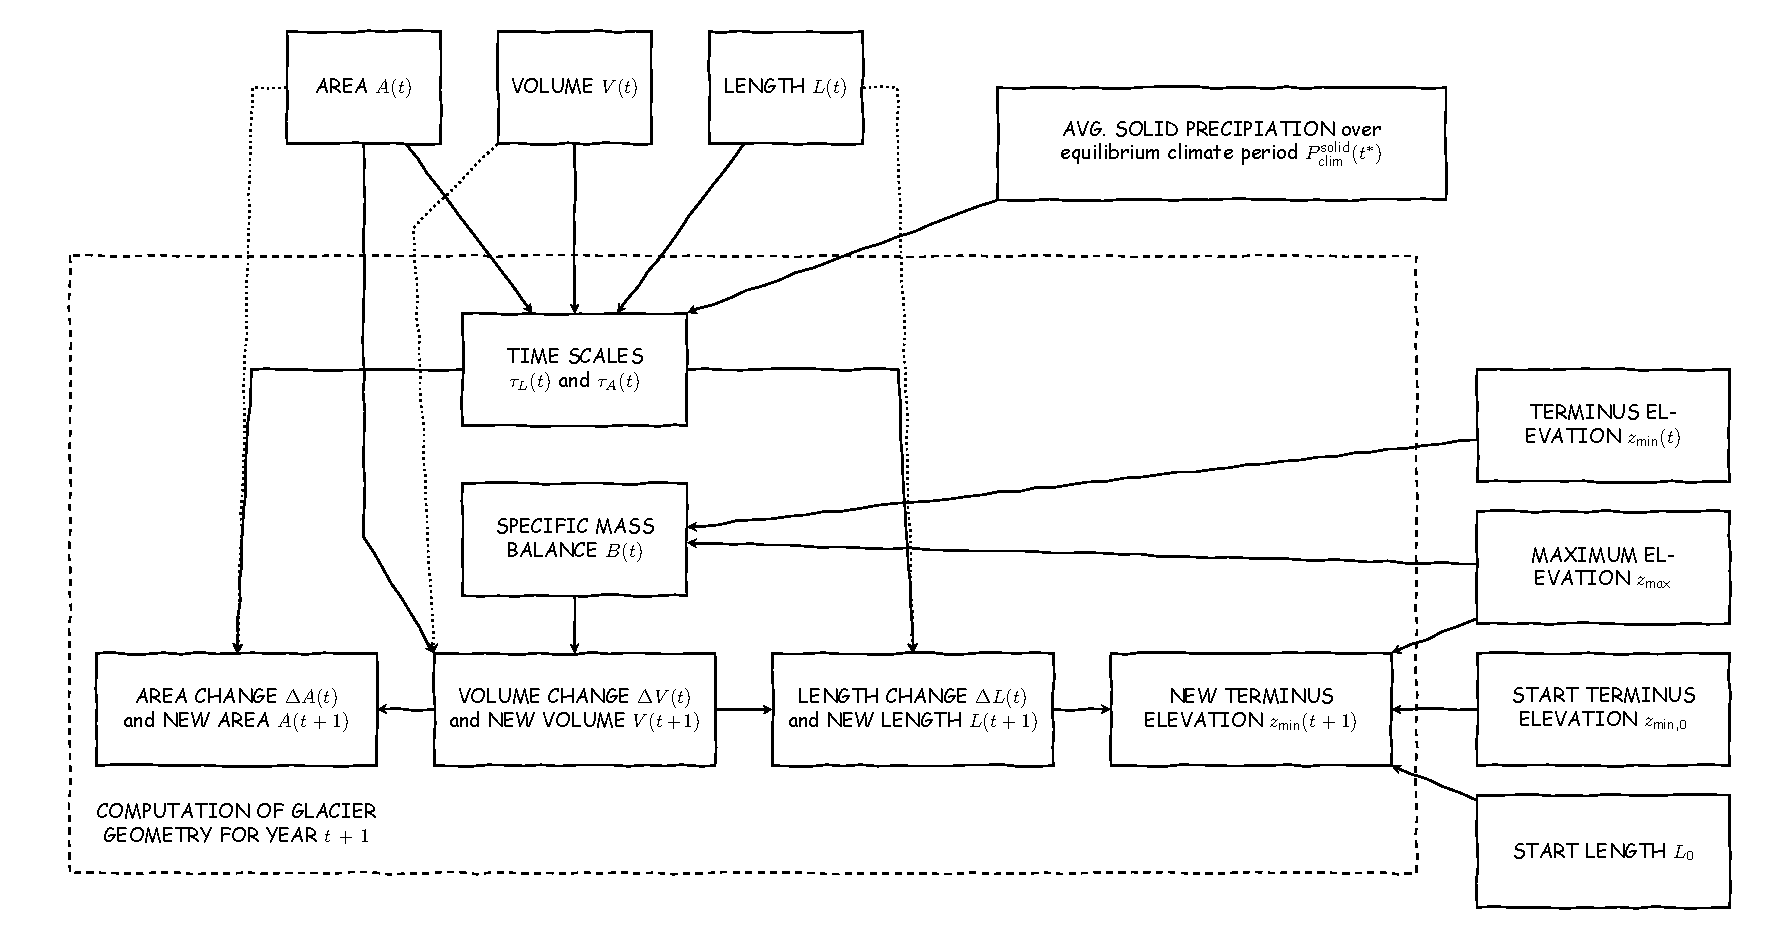
\includegraphics[width=0.65\textwidth]{/Users/oberrauch/work/master/flowchart/iterations/scaling.pdf}
    
    \end{frame}

    \begin{frame}[t]\frametitle{Volume/area scaling model}
        
        \onslide<1->{
        Volume changes instantaneously:
        \begin{align*}
            \Delta V(t) = \frac{1}{\rho_\text{ice}} A(t)\cdot B(t)
        \end{align*}}
        
        \onslide<2->{
        \vfill
        Area and length follow \textbf{response time scaling}:
        \begin{align*}
            \Delta L(t) &= \frac{1}{\tau_L}\left(\left(\frac{V(t)}{c_L}\right)^{1/q} - L(t) \right)\\[12pt]
            \Delta A(t) &= \frac{1}{\tau_A}\left(\left(\frac{V(t)}{c_A}\right)^{1/\gamma} - A(t) \right)
        \end{align*}}
    
    \end{frame}


    \begin{frame}[t]\frametitle{Hintereisferner test case}
        \centering
        \only<1>{Relative ice volume:\\[20pt]
        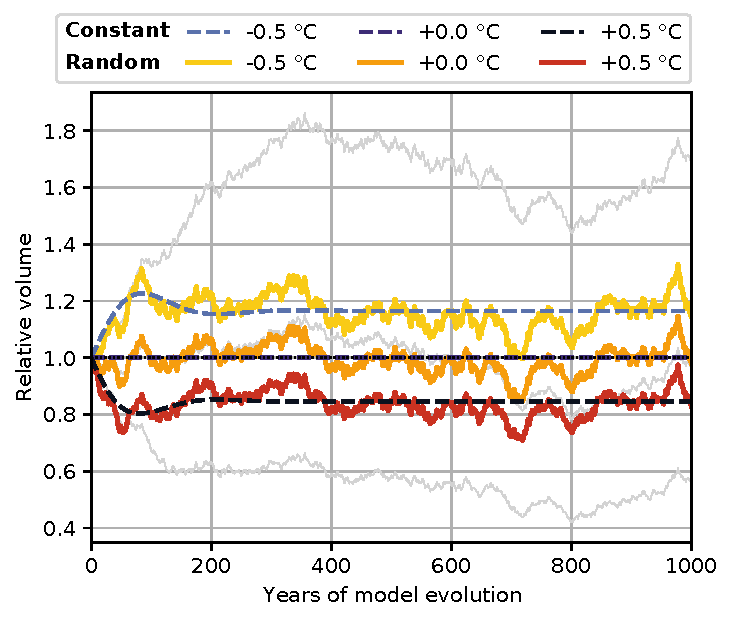
\includegraphics[width=0.49\textwidth]{/Users/oberrauch/work/master/plots/final_plots/time_series/single_glaciers/volume_norm_vas_Hintereisferner.pdf}
        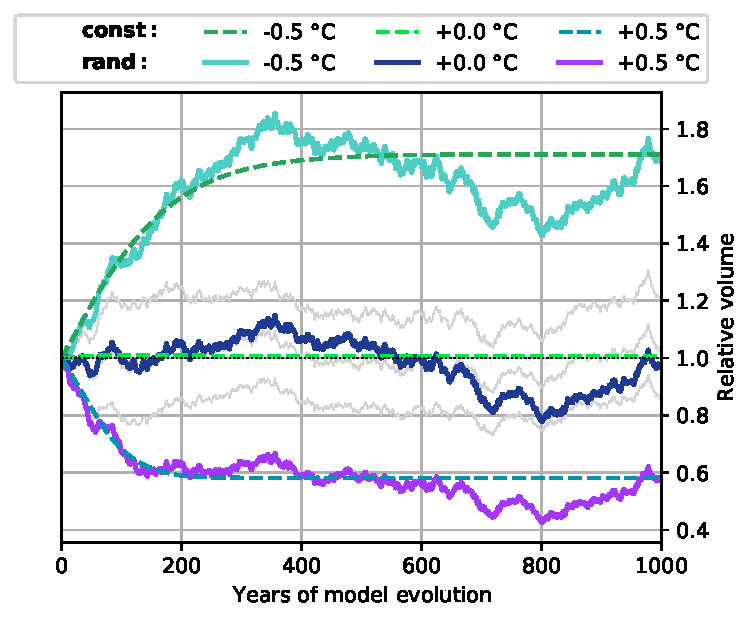
\includegraphics[width=0.49\textwidth]{/Users/oberrauch/work/master/plots/final_plots/time_series/single_glaciers/volume_norm_fl_Hintereisferner.pdf}}
        
        \only<2>{Relative surface area:\\[20pt]
        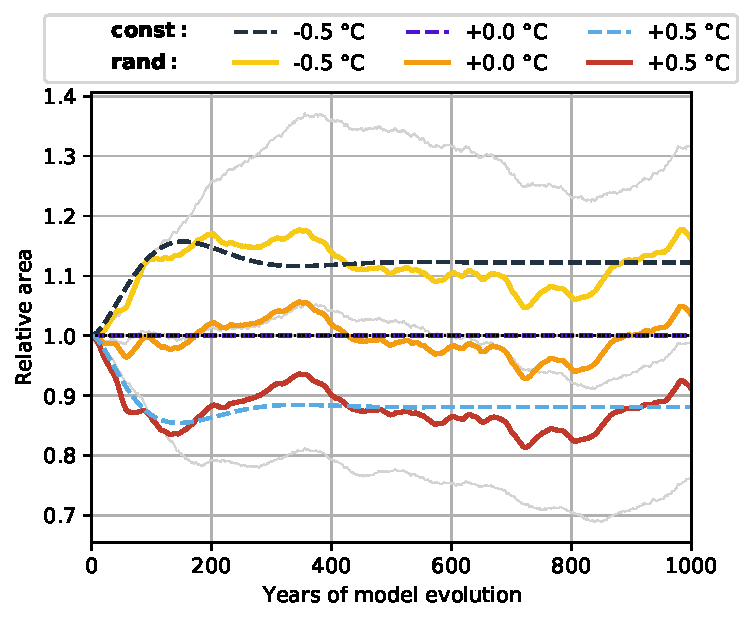
\includegraphics[width=0.49\textwidth]{/Users/oberrauch/work/master/plots/final_plots/time_series/single_glaciers/area_norm_vas_Hintereisferner.pdf}
        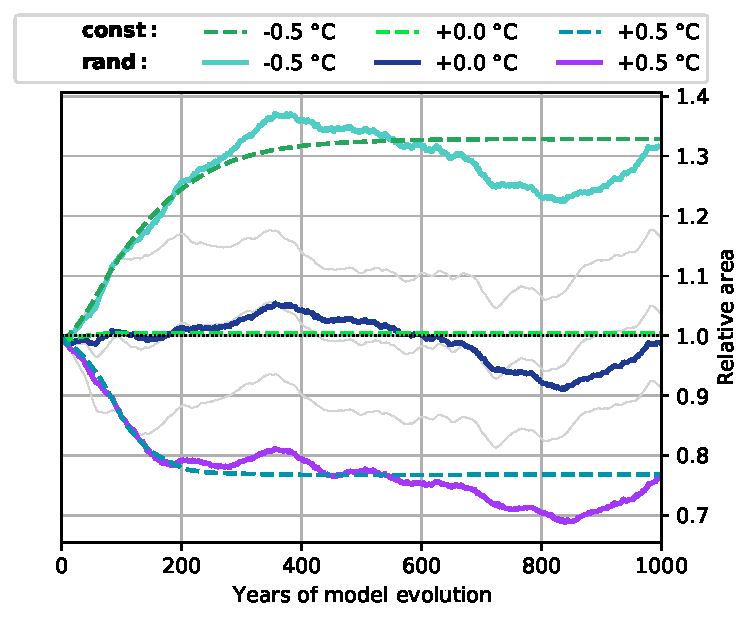
\includegraphics[width=0.49\textwidth]{/Users/oberrauch/work/master/plots/final_plots/time_series/single_glaciers/area_norm_fl_Hintereisferner.pdf}}

        \only<3>{Relative glacier length:\\[20pt]
        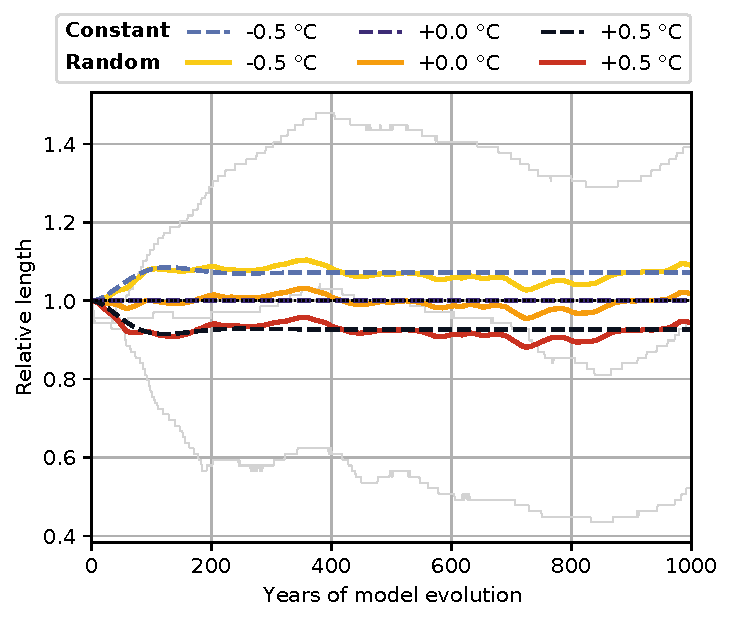
\includegraphics[width=0.49\textwidth]{/Users/oberrauch/work/master/plots/final_plots/time_series/single_glaciers/length_norm_vas_Hintereisferner.pdf}
        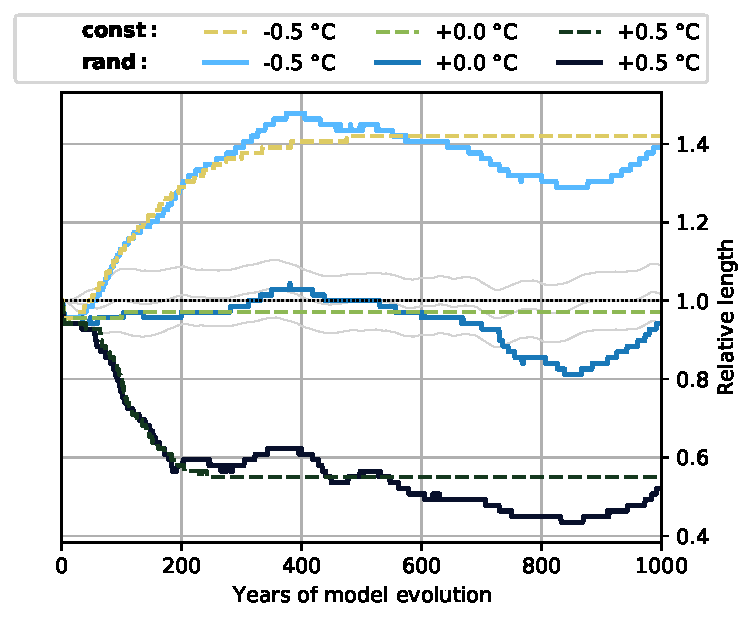
\includegraphics[width=0.49\textwidth]{/Users/oberrauch/work/master/plots/final_plots/time_series/single_glaciers/length_norm_fl_Hintereisferner.pdf}}
    
    \end{frame}

    \begin{frame}[t]\frametitle{Power spectral density}
        \centering
        \only<1>{HEF - Length under random climate:\\[12pt]
        \includegraphics[width=0.65\textwidth]{/Users/oberrauch/work/master/plots/final_plots/random_length/Hintereisferner.pdf}}
        \only<2>{HEF - Power spectral density:\\[12pt]
        \includegraphics[width=0.65\textwidth]{/Users/oberrauch/work/master/plots/final_plots/psd/Hintereisferner.pdf}}
    
    \end{frame}

    \begin{frame}[t]\frametitle{Autocorrelation function}
        \centering
        \only<1>{HEF - Autocorrelation function:\\[12pt]
        \includegraphics[width=0.65\textwidth]{/Users/oberrauch/work/master/plots/final_plots/acf/Hintereisferner.pdf}}
        \only<2>{HEF - Partial autocorrelation function:\\[12pt]
        \includegraphics[width=0.65\textwidth]{/Users/oberrauch/work/master/plots/final_plots/pacf/Hintereisferner.pdf}}
    
    \end{frame}


    \begin{frame}[t]\frametitle{HISTALP domain}
        \centering
        \only<1>{Relative ice volume:\\[20pt]
        \includegraphics[width=0.49\textwidth]{/Users/oberrauch/work/master/plots/final_plots/time_series/histalp_commitment/volume_norm_vas.pdf}
        \includegraphics[width=0.49\textwidth]{/Users/oberrauch/work/master/plots/final_plots/time_series/histalp_commitment/volume_norm_fl.pdf}}
       
    
    \end{frame}


    \begin{frame}[t]\frametitle{Sensitivity experiments}
        \centering
        \only<1>{Hintereisferner:\\[20pt]
        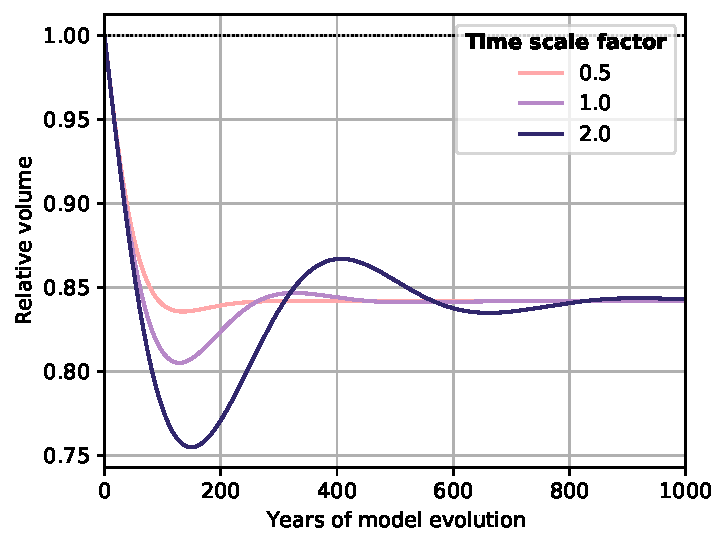
\includegraphics[width=0.49\textwidth]{/Users/oberrauch/work/master/plots/final_plots/sensitivity/time_scales_hef.pdf}
        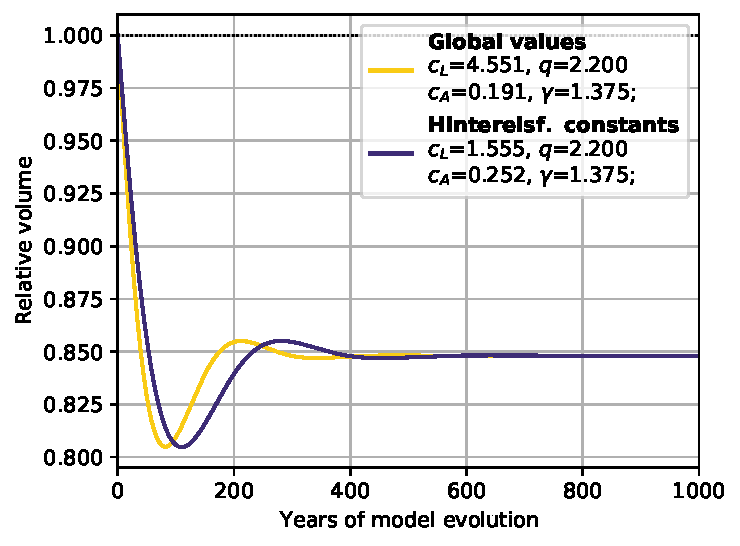
\includegraphics[width=0.49\textwidth]{/Users/oberrauch/work/master/plots/final_plots/sensitivity/scaling_params_hef.pdf}}
        \only<2>{HISTALP domain:\\[20pt]
        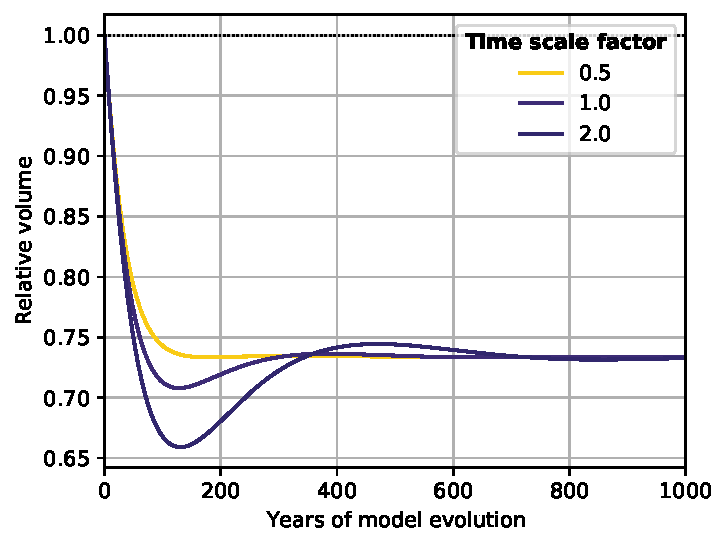
\includegraphics[width=0.49\textwidth]{/Users/oberrauch/work/master/plots/final_plots/sensitivity/time_scales_histalp.pdf}
        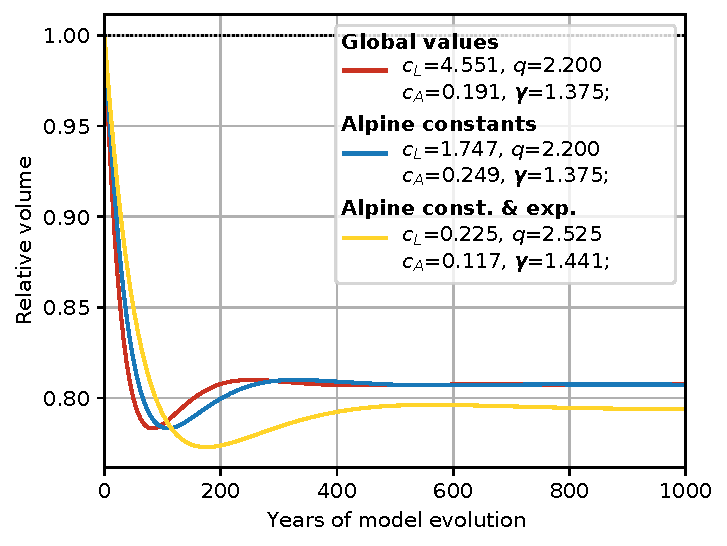
\includegraphics[width=0.49\textwidth]{/Users/oberrauch/work/master/plots/final_plots/sensitivity/scaling_params_histalp.pdf}}
       
    
    \end{frame}


	\begin{frame}[t]\frametitle{Future projection}
        \centering
        \only<1>{Relative ice volume:\\[20pt]
        \includegraphics[width=0.49\textwidth]{/Users/oberrauch/work/master/plots/final_plots/time_series/histalp_projection/volume_norm_vas.pdf}
        \includegraphics[width=0.49\textwidth]{/Users/oberrauch/work/master/plots/final_plots/time_series/histalp_projection/volume_norm_fl.pdf}}
       
    
    \end{frame}

    \begin{frame}[t]\frametitle{Take Home Message}
        \vfill
        \textbf{Volume/area scaling model characteristics:}
        \begin{itemize}
            \item<1->Underestimates volume and volume changes
            \item<2->Correctly depicts low pass filter
            \item<3->Short(er) response times
            \item<4->Response of a damped oscillator
            \item<5->Weak sensitivity to scaling parameters
        \end{itemize}

        \begin{block}{\color[HTML]{f69d0e}{(Maybe) not up to date, anymore.}}<6->
        
        \end{block}
        
    
    
    \end{frame}

    \begin{frame}[t]\frametitle{Crossvalidation}
        \centering
        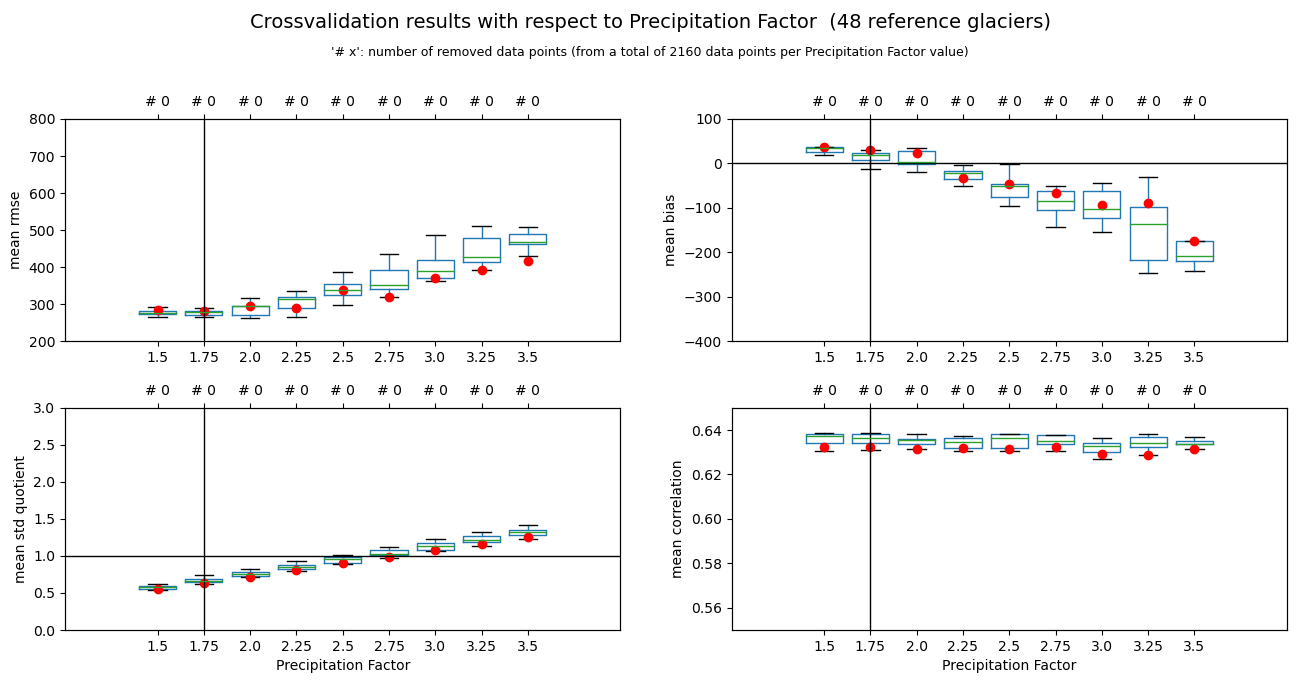
\includegraphics[width=\textwidth, ]{/Users/oberrauch/mb_crossval/data/xval/http/1.1.2.dev44+gf9ab669-histalp/plots/prcpsf_crossval_box.png}
        
    
    \end{frame}

	% bibliography
    \begin{frame}[t]\frametitle{References}
        \bibliographystyle{ametsoc.bst}
        \bibliography{../thesis/master.bib}
    \end{frame}
	

\end{document}
